
\section{The trigger}
\label{ss:secTrig}
At the LHC, the proton beams are made to collide after 25\unit{ns}. Due to such a high
collision rate a huge number of events, roughly 40 million, are produced at
every second. Storing all these events would require many petta bytes
(1\unit{PB} = 1000000\unit{GB}) of computer memory, which is practically not possible as the
collision happens over a large period of time (many months). Even if somehow one 
can get around this challenge, most of the events are produced from soft collision 
and contain no interesting physics process. To filter events which are of physics 
interest, a two-tier trigger system is deployed at the CMS experiment. The first is 
called Level-1 (L1) trigger which is based on hardware (by collecting information from 
various sub-detectors) and the second is called High Level Trigger (HLT) which 
is based on software algorithms. The event rate after passing through these 
triggers are shown in Table~\ref{tab:trigRate}. After applying the HLT, the 
event rate is reduced to 200\unit{Hz} which requires about 200\unit{MB} of computer memory. 
A brief description of the L1 and HLT triggers are given in this thesis. A detailed 
description of these can be found in Reference~\cite{Khachatryan:2016bia}.
\begin{table}
\caption{\label{tab:trigRate} Event rate after applying level-1 and high-level
	triggers.}
\begin{centering}
\begin{tabular}{cccc}
\hline
\hline
\noalign{\vskip 0.1cm}
	Input event rate & Trigger & Type & Output event rate 
\tabularnewline
\hline
\hline
\noalign{\vskip 0.1cm}
	40\unit{MHz} & L1   & Hardware & 100\unit{KHz} \tabularnewline
\noalign{\vskip 0.1cm}
	100\unit{KHz} & HLT & Software & 200\unit{Hz} \tabularnewline
\hline
\end{tabular}
\par\end{centering}
\end{table}


\begin{itemize} [leftmargin=*]
\item \textbf{Level-1 Trigger}: L1 is also called online trigger as 
events are triggered during the data taking. The L1 trigger is 
required to be very fast with a latency of 4\unit{$\mu$s}. The decision to either 
keep or reject events by this trigger is based on a set of information 
provided by various sub-detectors as shown in Figure~\ref{fig:L1Trig}.
Over 8000 towers of the calorimeters (ECAL and HCAL) send transverse energies
and quality flags to the regional calorimeter trigger (RCT). These pieces of
information are processed in parallel by the RCT. The $e/\gamma$ candidates along 
with $E_{T}$ sums based on $4\times 4$ towers are sent by RCT to the global calorimeter
trigger (GCT). The GCT finds central-jets, forward-jets, tau-jets, and missing transverse energy.
The decision based on the findings of GCT is conveyed to the global trigger (GT) 
whether to keep an event or not. The other decision conveyed to the GT comes 
from the global muon trigger (GMT). The GMT takes input from different muon chambers.
The hits from RPC is sent to the pattern comparator (PC) which finds muon 
candidates. The information about the number of muon candidates from the PC is 
shared with the GMT. The front-end trigger electronics identify segments from 
the hits in CSC and DT. These segments are sent to the regional track finder (TF).
In the TF, the PC comparator identifies muon candidates and measures momentum 
from the bending of tracks due to the magnetic field. The muon candidates with the
corresponding momentum from the TF are shared with GMT. The GMT decides whether
an event is worth keeping from muon's point of view. Finally, the collective
decision from the GCT and GMT is passed to the global trigger which takes
the final call. The decision of the GT is conveyed to the data acquisition system 
(DAQ) which stores data from sub-detectors such as tracker (TRK), ECAL, HCAL, and muon 
chambers. If the event is going to be rejected by the GT then the DAQ does not 
store corresponding data from the sub-detectors.
\begin{figure}
  \begin{center}
  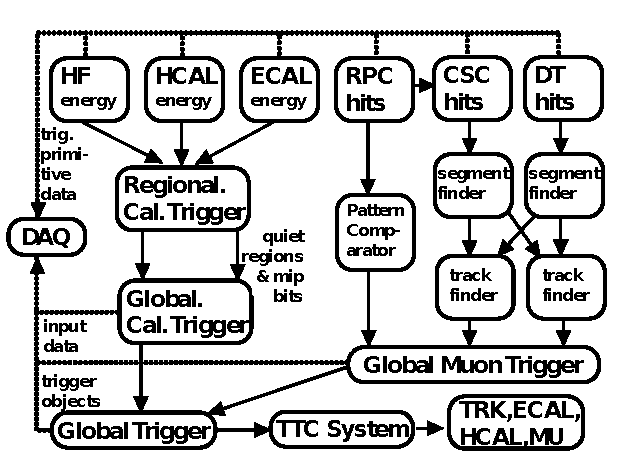
\includegraphics[width=0.70\linewidth]{Experiment/CMS/Image/L1Trig.pdf}
  \caption{Workflow of decisions for the Level-1 trigger \cite{Khachatryan:2016bia}.}
  \label{fig:L1Trig}
  \end{center}
\end{figure}

\item \textbf{High Level Trigger}: After applying L1 trigger, the filtered events
are passed as input to the HLT. The L1 bits available in the event serve
as the seed for HLT. The decision to reject or keep an event from the HLT
is taken based on whether an event has a reasonable number of physics objects
such as electrons, muons, and jets  with transverse momentum above some
threshold. In order to reconstruct these physics objects, a set of dedicated
software algorithms is run for every event. During the run, the input from one 
step is passed to the subsequent steps. For every event, the HLT decision is 
stored in the form of programming strings also called trigger paths. 

The HLTs are applied to select events enriched
with desired physics objects. Depending on the topology of analysis, an 
event is selected if the corresponding trigger path is available in that 
event. In this thesis, we have 1 lepton, at least 4 jets, and neutrino in the 
final state. Therefore, an event is selected if it has a trigger 
path of \verb|HLT_IsoMu24*| and \verb|HLT_IsoTkMu24*| with logical \verb|OR| 
for the muon channel, and \verb|HLT_Ele27_WPTight_Gsf| for the electron 
channel. Having these muon trigger paths in the event ensures that there is at least one 
isolated muon with \pt more than 24 \GeV (see Section~\ref{s:muReco}) whereas
the electron trigger path implies the presence of at least one electron with \pt 
more than 27 \GeV with tight working point (WP) reconstructed with Gaussian sum 
filter algorithm (see Section~\ref{s:eleReco}). The efficiency of these triggers depends on 
\pt and $\eta$ of the lepton. For lower \pt, the efficiency is very poor and has 
a sudden increase at a particular value. That sudden increase is called trigger 
turn-on and the leptons are required to have a \pt greater than that at the turn-on.

The muon and electron trigger efficiency as a function of \pt is shown 
in Figure~\ref{fig:trigEff}. The trigger turn-on for muon trigger is 
at about \pt = 24 \GeV, hence in the subsequent selection (Section~\ref{s:muReco}),
the muon is required to have \pt $>$ 26 \GeV. For the electron trigger 
(\verb|HLT_Ele27_WPTight_Gsf|), the trigger turn-on is at around 
\pt = 33 \GeV, therefore a cut of \pt $>$ 35 \GeV is applied on 
electrons in the subsequent selection (Section~\ref{s:eleReco}).
\begin{figure}
\centering
\subfigure[Muon trigger efficiency \cite{ref:muon-twiki}]
{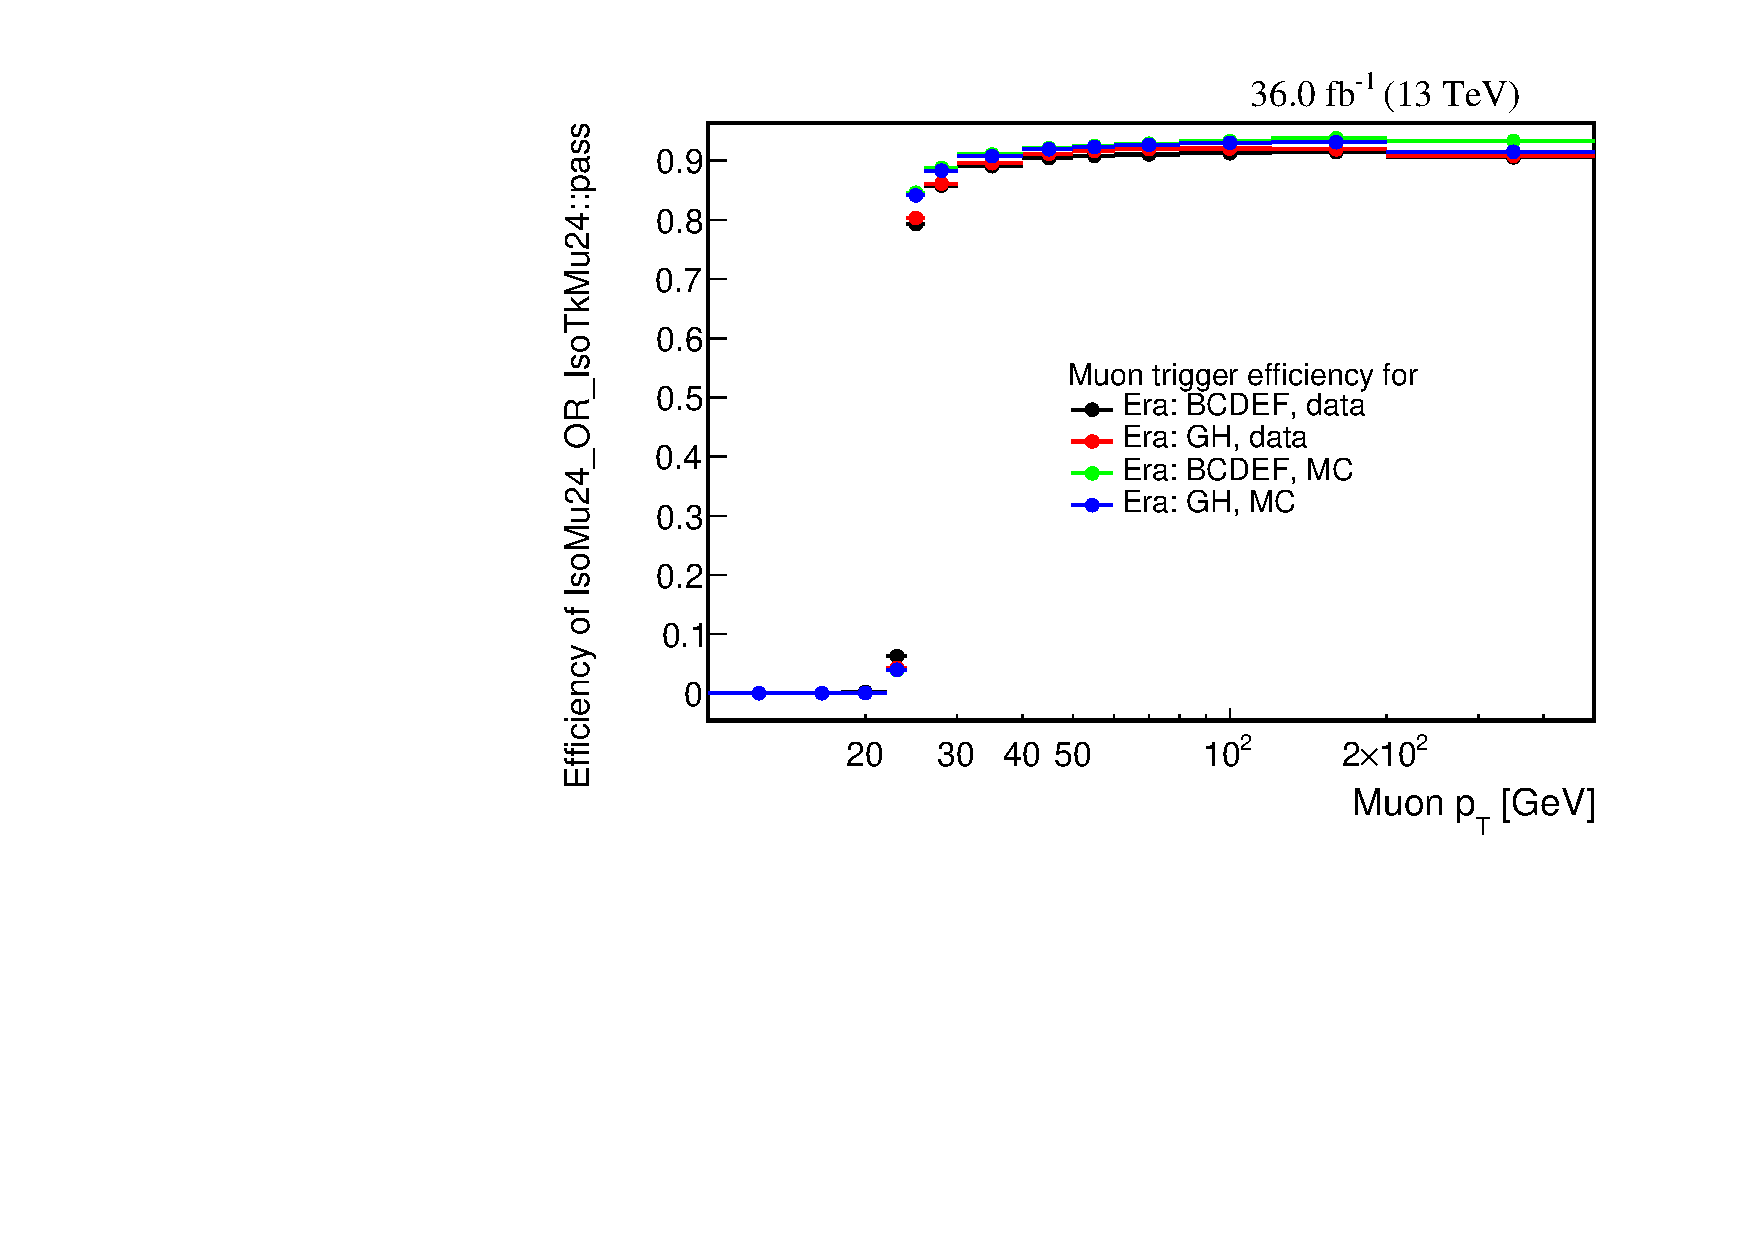
\includegraphics[width=0.60\linewidth]{Image/Muon/muSF_png/muonTrigEff.pdf}}
\vfil
\subfigure[Electron trigger efficiency in the barrel region \cite{eleTrigEff}]
{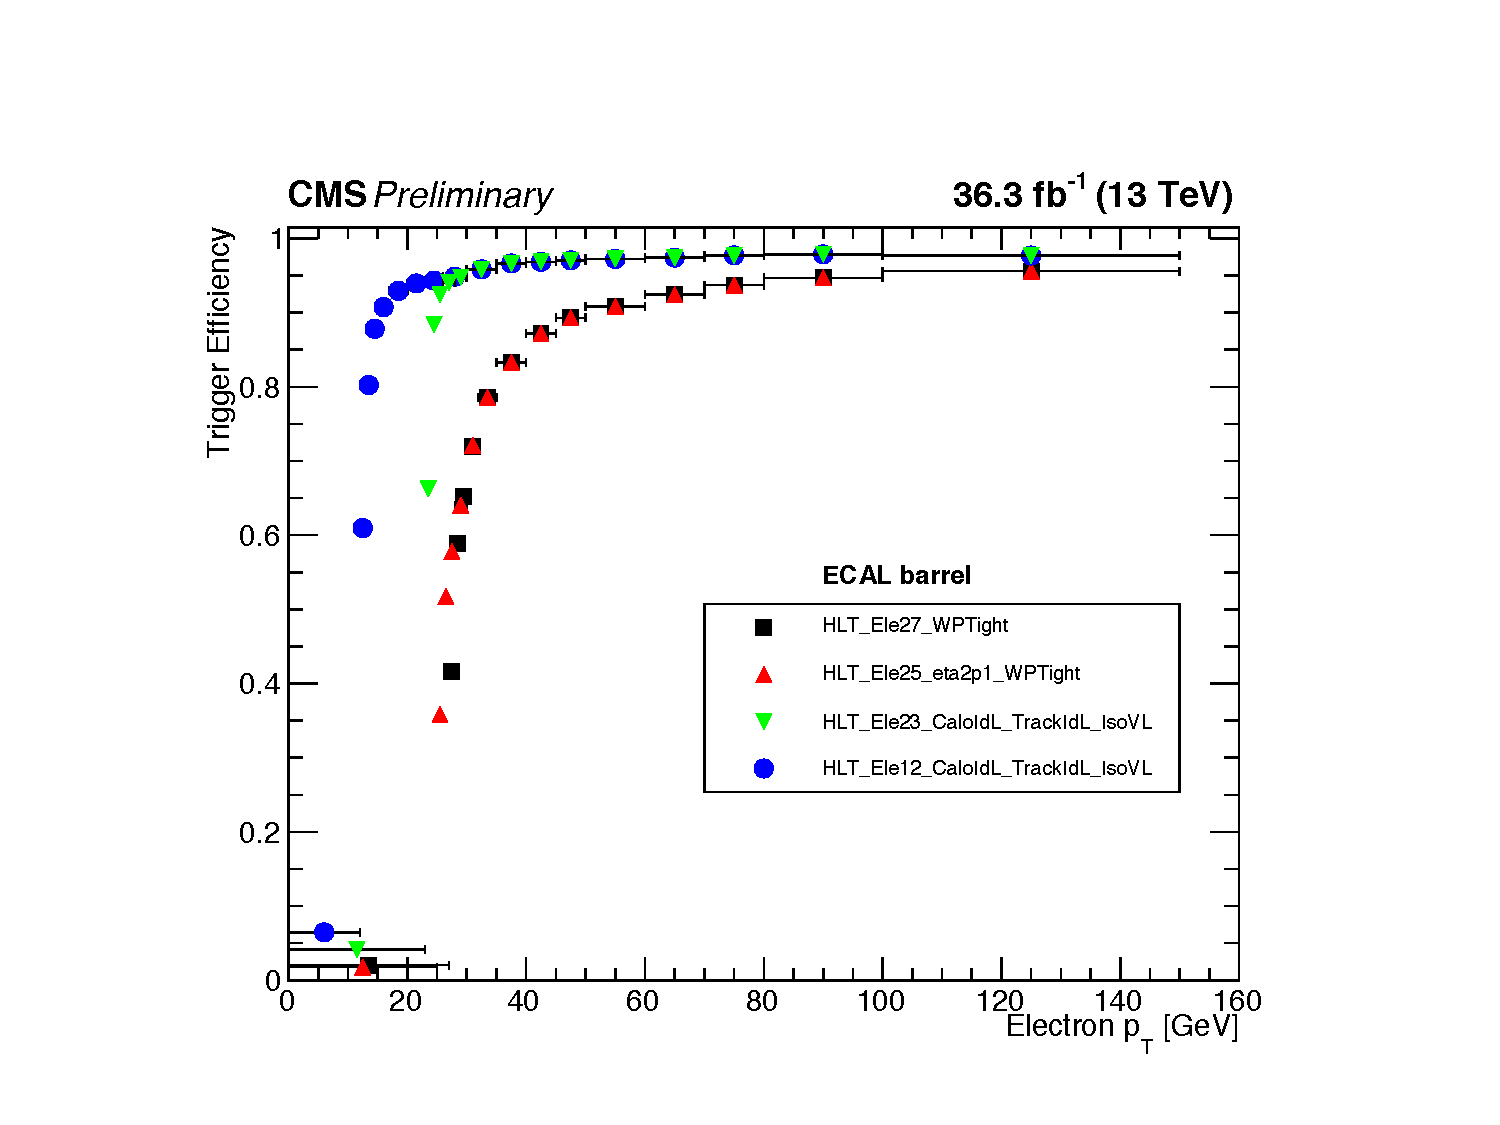
\includegraphics[width=0.49\linewidth]{Image/Electron/eleSF_png/eleTrigEB.pdf}}
\subfigure[Electron trigger efficiency in the endcap region \cite{eleTrigEff}]
{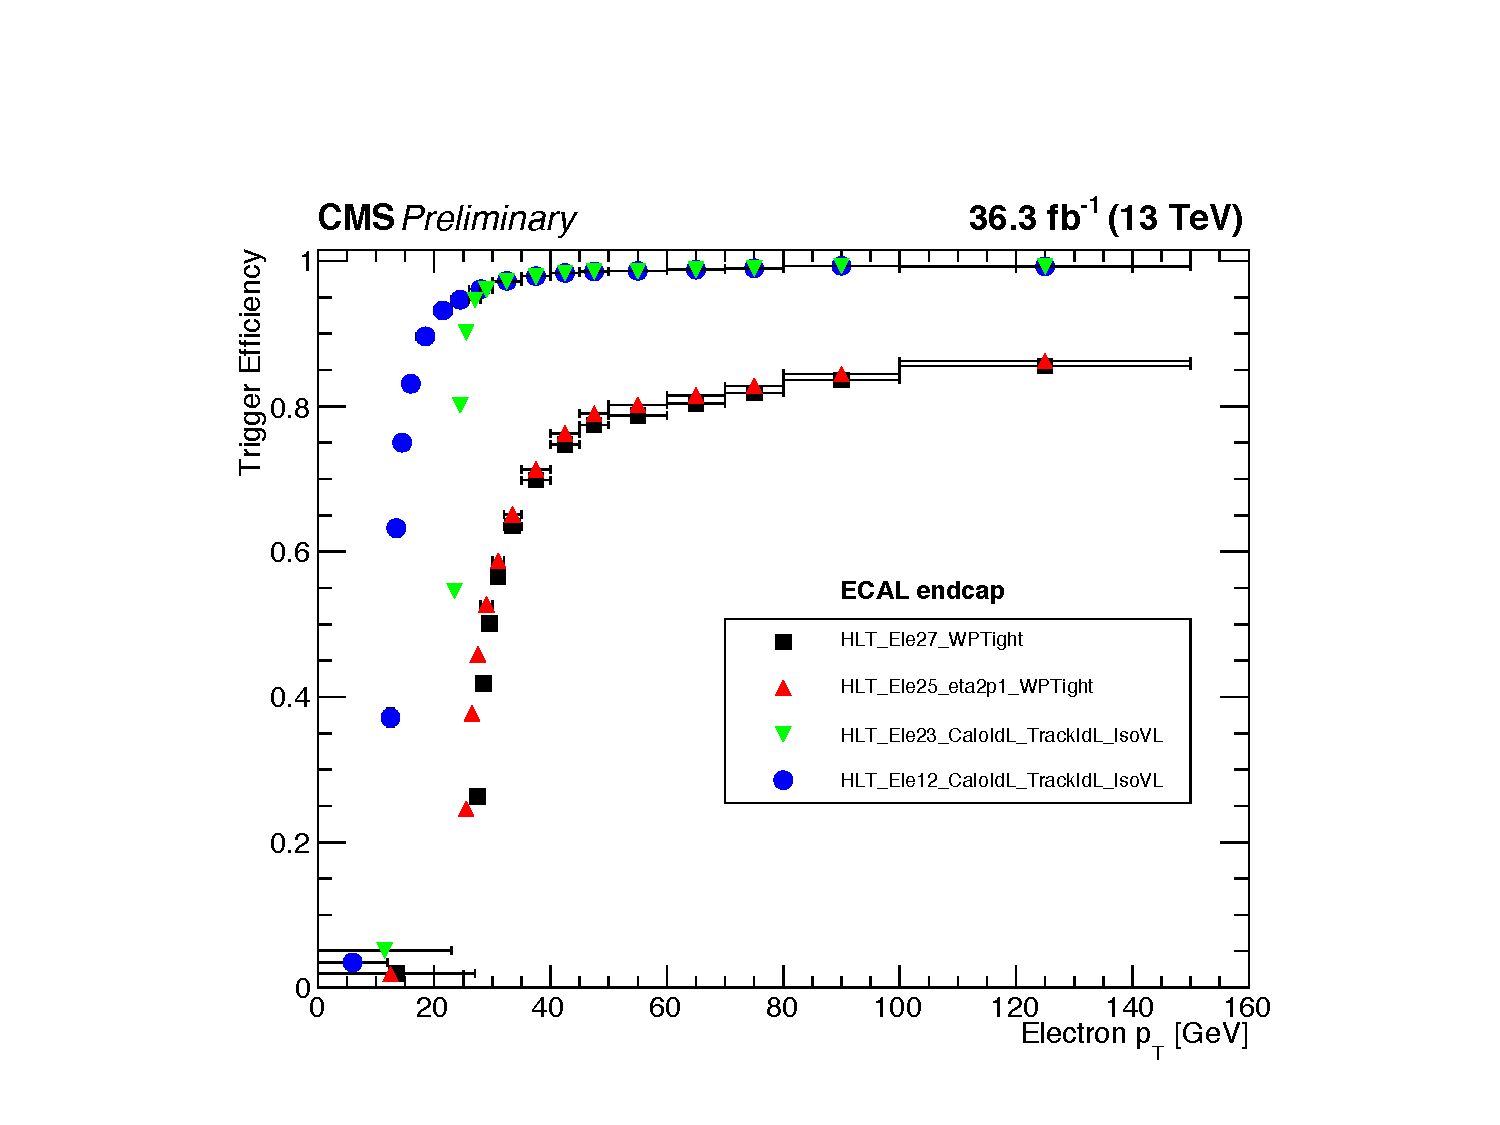
\includegraphics[width=0.49\linewidth]{Image/Electron/eleSF_png/eleTrigEE.pdf}}
\caption{Muon and electron trigger efficiency as a function of \pt. 
The trigger turn-on is at about \pt = 24 \GeV for muon, and 33 \GeV for electron trigger.}
\label{fig:trigEff}
\end{figure}
\end{itemize}

